\section{Systèmes existants}
De nos jours, on retrouve sur le marché international, une variété de systèmes ANPR commerciaux tels que:
    \begin{itemize}
        \item[•]\textbf{AutoVu}: c’est le système de \acrfull{rapi} sur IP de Security Center qui automatise la lecture et vérification de plaques d'immatriculation de véhicules. Il utilise des caméras qui capturent des images de plaques et transmettent les données à un Patroller ou Security Center, qui recherche la plaque dans des listes de véhicules recherchés ou de permis. \cite{autoVu}
            \begin{figure}[H]
                \centering
                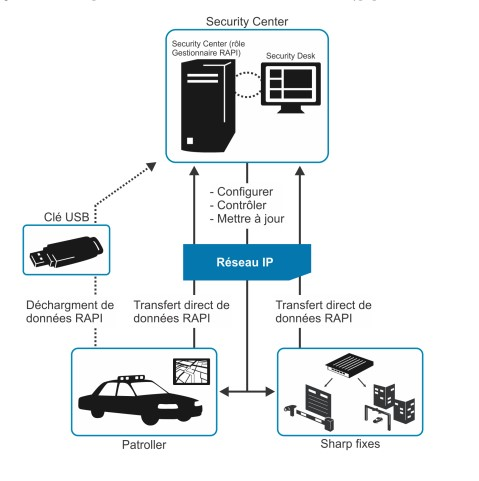
\includegraphics[scale=0.4]{autoVu}
                \caption{Fonctionnement d'un réseau AutoVu typique}
            \end{figure}  
        \item[•]\textbf{LAPI ENGINE}: C’est un OCR de lecture de plaques d'immatriculation permettant d'identifier et de tracer les véhicules passant sur une zone et se présentant devant une caméra, à partir d'un flux vidéo en direct ou de séquences vidéo d'évènements détectés par les caméras. \cite{lapiWeb, lapiManual}
        \begin{figure}[H]
            \centering
            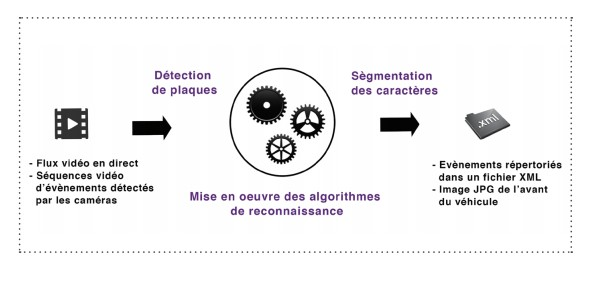
\includegraphics[scale=0.6]{lapiEngine}
            \caption{Schéma fonctionnel du LAPI Engine}
        \end{figure} 
        \item[•] En plus des systèmes cités plus haut, nous avons d'autres comme les \textbf{caméras de contrôle de vitesse \textit{TrajectControle}} qui sont implémentées au Pays-Bas depuis 2002, les \textbf{systèmes de reconnaissance \textit{Zamir Ltd}} de Jérusalem en Israël, \textbf{\textit{SeeTec}}, \textbf{\textit{Asia Vision Technology Limited}} et bien d'autres encore. \cite{HindeThesis, NorMaster}
    \end{itemize} 
    